\RequirePackage[hyphens]{url}
\documentclass[hidelinks,a4paper]{article}
\usepackage[top=0.1in, bottom=0.1in, left=0.1in, right=0.1in]{geometry}
\usepackage{amsmath}
\usepackage{graphicx}
\usepackage{url}
%\usepackage[hyphens]{url}
\usepackage{hyperref}
\usepackage{breakurl}
\usepackage{setspace}
\usepackage{array}
\usepackage{amssymb}
\usepackage[mathscr]{euscript}
%\renewcommand{\rmdefault}{bch} % change default font
\usepackage{tikz}
\usetikzlibrary{calc}
\usetikzlibrary{shapes}
\usepackage{enumitem}
\setlength{\parindent}{0in}
\usepackage{bm}
\usepackage{multirow}
\usepackage{adjustbox}
\usepackage{scalerel}
\usepackage[many]{tcolorbox}
\usepackage{booktabs}
%\usepackage{adjustbox}
%>{\centering\arraybackslash}m{3cm}
%\newcolumntype{Y}{>{\small\raggedright\arraybackslash}X}
%\newcolumntype{C}{>{\centering\arraybackslash}m{3cm}}
\newcolumntype{C}{>{$}c<{$}}
%\captionsetup{
%	justification = centering
%}

\newcommand{\myfrac}[2]{\displaystyle \frac{#1}{#2}}
\newcommand{\dsum}{\displaystyle \sum}
%\newcommand{\mystrut}{\rule[10pt]{10pt}{20pt}}
\newcommand{\mystrut}{\rule[1\dp\strutbox]{0pt}{\baselineskip}}
\newcommand{\mysup}[1]{\scaleto{\rule[2.9\dp\strutbox]{0pt}{-1\baselineskip}^{#1}}{12pt}}
\newcommand{\mysub}[1]{\scaleto{\rule[-1.5\dp\strutbox]{-2.5pt}{-1\baselineskip}_{#1}}{5pt}}

\doublespacing
\pagenumbering{gobble}
\begin{document}

\begin{center}
	\begin{table}[!ht]
		%\footnotesize
		\fontsize{14.5}{17.4}\selectfont
		\setlength{\tabcolsep}{4pt}
		\setlength\arrayrulewidth{1.5pt}
		
		\centering
		%\caption{Summary of all asymptotic distance distributions for each metric.}
		\label{table:distribution_summary}
		\begin{adjustbox}{max width=\textwidth}
		\begin{tabular}[c]{|c|c|c|@{}m{0pt}@{}} \hline
		& & & \\ [-2.3ex]
        {\huge \textbf{Type}}      & {\huge \textbf{Mean}}                & {\huge \textbf{Variance}}                & \\ [1ex] \hline \hline
        $\mathcal{N}(0,1)-\bm{\textbf{d}_{\textbf{M}}}$ & $\dfrac{2p}{\sqrt{\pi}}$       & $\dfrac{2p(\pi - 2)}{\pi}$         & \\ [4ex]  \hline 
        $\mathcal{N}(0,1)-\bm{\textbf{d}^{*}_{\textbf{M}}$}   & 
           {\begin{tabular}{c}
           	    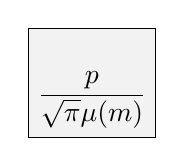
\begin{tikzpicture}
                \node[draw,fill=black!5!,text height=0.82cm] (label) {$\dfrac{p}{\sqrt{\pi} \mu(m)}$};
                \end{tikzpicture} \\ [2ex]         
        	    where \hspace{0.2cm} $\mu(m) = \dfrac{\text{log}(\text{log}(2))}{\Phi^{-1}\left(\frac{1}{m}\right)} - \Phi^{-1}\left(\frac{1}{m}\right)$
           \end{tabular}} &         
          {\begin{tabular}{c}
        	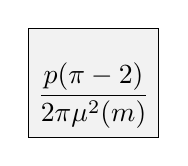
\begin{tikzpicture}
        	   \node[draw,fill=black!5!,text height=0.82cm] (label) {$\dfrac{p(\pi - 2)}{2\pi\mu^2(m)}$};
            \end{tikzpicture} \\ [2ex]
            where \hspace{0.2cm} $\mu(m) = \dfrac{\text{log}(\text{log}(2))}{\Phi^{-1}\left(\frac{1}{m}\right)} - \Phi^{-1}\left(\frac{1}{m}\right)$
          \end{tabular}} & \\ [15ex] \hline
        $\mathcal{N}(0,1)-\bm{\textbf{d}_{\textbf{E}}$} & $\sqrt{2p-1}$                  & 1                                & \\ [5ex]  \hline
        $\mathcal{N}(0,1)-\bm{\textbf{d}^{*}_{\textbf{E}}$}   &
        {\begin{tabular}{c}
               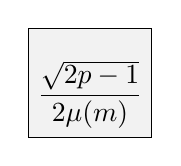
\begin{tikzpicture}
               \node[draw,fill=black!5!,text height=0.82cm] (label) {$\dfrac{\sqrt{2p-1}}{2\mu(m)}$};
               \end{tikzpicture} \\ [2ex]
               where \hspace{0.2cm} $\mu(m) = \dfrac{\text{log}(\text{log}(2))}{\Phi^{-1}\left(\frac{1}{m}\right)} - \Phi^{-1}\left(\frac{1}{m}\right)$
         \end{tabular}} &
        {\begin{tabular}{c}        
               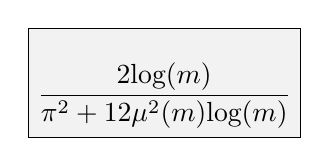
\begin{tikzpicture}
        	   \node[draw,fill=black!5!,text height=0.82cm] (label) {$\dfrac{2\text{log}(m)}{\pi^2 + 12\mu^2(m)\text{log}(m)}$};
               \end{tikzpicture} \\ [2ex]
        	   where \hspace{0.2cm} $\mu(m) = \dfrac{\text{log}(\text{log}(2))}{\Phi^{-1}\left(\frac{1}{m}\right)} - \Phi^{-1}\left(\frac{1}{m}\right)$
         \end{tabular}} & \\ [15ex]  \hline
        $\mathcal{U}(0,1)-\bm{\textbf{d}_{\textbf{M}}$} & $\dfrac{p}{3}$                 & $\dfrac{p}{18}$                   & \\ [5ex]  \hline
        $\mathcal{U}(0,1)-\bm{\textbf{d}^{*}_{\textbf{M}}$}   & $\dfrac{(m+1)p}{3(m-1)}$       & $\dfrac{(m^3-18m^2-5m+2)p}{18(m^3+m^2+2)(m-1)^2}$ & \\ [5ex] \hline
        $\mathcal{U}(0,1)-\bm{\textbf{d}_{\textbf{E}}$} & $\sqrt{\dfrac{p}{6} - \dfrac{7}{120}}$ & $\dfrac{7}{120}$           & \\ [5ex]  \hline
        $\mathcal{U}(0,1)-\bm{\textbf{d}^{*}_{\textbf{E}}$}   & $\sqrt{\dfrac{p}{6} - \dfrac{7}{120}} \left(\dfrac{m+1}{m-1}\right)$ & $\dfrac{7(m+1)^2(m+2)}{120(m^3+m^2+2)}$ & \\ [5ex] \hline
		\end{tabular}
	\end{adjustbox}
	\end{table}
\end{center}

\end{document}